\documentclass[a4paper, 12pt]{article}

\usepackage{geometry}
\geometry{left=2cm, right=2cm, top=2cm, bottom=2cm}

\usepackage{cmap}
\usepackage{mathtext} 
\usepackage[T2A]{fontenc}
\usepackage[utf8]{inputenc}
\usepackage[english,russian]{babel}	

\usepackage{amsfonts,amssymb,amsthm,mathtools}
\usepackage{amsmath}
\usepackage{icomma} 

\usepackage{graphicx} 
\graphicspath{{picturies/}}
\usepackage{wrapfig}

\usepackage{array,tabularx,tabulary,booktabs}
\usepackage{longtable}
\usepackage{multirow}

\usepackage{caption}
\captionsetup{labelsep=period}

\renewcommand{\phi}{\varphi}
\newcommand{\eps}{\varepsilon}
\newcommand{\parag}[1]{\paragraph*{#1:}}

\newcounter{Points}
\setcounter{Points}{1}
\newcommand{\point}{\arabic{Points}. \addtocounter{Points}{1}}

\author{Радькин Кирилл, Б01-005}
\date{7.05.22}
\title{Лабораторная работа 4.3.3. Исследование разрешающей способности микроскопа методом Аббе.}

\begin{document}
\maketitle
\thispagestyle{empty}

\textbf{\\Цель работы:} изучение дифракционного предела разрешения объектива микроскопа.
\\\\
\textbf{В работе используются:} лазер; кассета с набором сеток разного периода; линзы; щель с микрометрическим винтом; оптический стол c набором рейтеров и крепёжных винтов; экран; линейка.
\\\\
\textbf{Схема установки:}

\begin{figure}[!h]
    \centering
    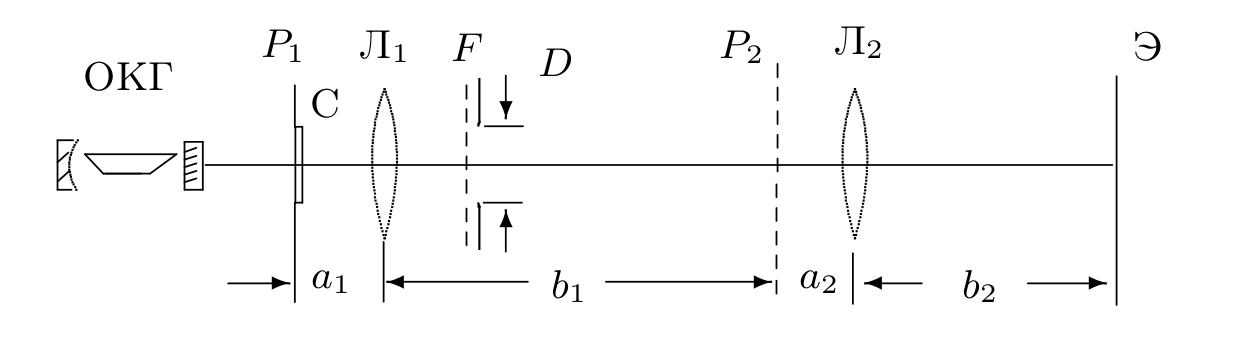
\includegraphics[scale = 0.3]{pic1.png}
    \caption{Схема экспериментальной установки~---~модель проекционного микроскопа}
    \label{pic1}
\end{figure}

\textbf{\\Теоретическое введение:}

\begin{itemize}
    \item Формула для расчета периодов решёток:
        \begin{equation*}
            d \sin \phi = m \lambda
        \end{equation*}

    \item Формула для расчета увеличения микроскопа:
        \begin{equation*}
            Г = \dfrac{b_1 b_2}{a_1 a_2}            
        \end{equation*}

    \item Формула для расчета минимального расстояния, разрешимого микроскопом:
        \begin{equation*}
            d \geq \dfrac{\lambda}{\left( D / 2f \right)} 
        \end{equation*}
\end{itemize}

\textbf{\\Ход работы:}

\begin{enumerate}
    \item Включим в сеть блок питания лазера.
    \item Закрепим кассету с решетками, пронаблюдаем дифракционные картины для разных сеток. Измерим расстояния между соседними дифракционными максимумами для каждой решетки.
    
        \begin{tabular}{|c|c|c|c|c|c|} \hline
            Номер решетки & 5 & 4 & 3 & 2 & 1 \\ \hline
            Расстояние, мм & 4.71 & 6.25 & 12.75 & 25.75 & 38.33 \\ \hline
        \end{tabular}

    \item Измерим расстояние от сетки до экрана $H = 1.40 \pm 0.01 м$
    \item Соберем модель проекционного микроскопа. 
    \item Определим расстояния $a_1 = 110 \pm 10$ мм, $a_2 = 25$ мм, $b_1 = 390 \pm 10$ мм, $b_2 = 1680 \pm 10$ мм
        Посчитаем увеличение микроскопа $Г = 238 \pm 22$
        Измерим периоды изображений сеток на экране:

        \begin{tabular}{|c|c|c|c|} \hline
            Номер решетки & 3 & 4 & 5 \\ \hline
            Период, мм & 4.41 & 8.33 & 11.0 \\ \hline
        \end{tabular}

    \item Поместим щелевую диафрагму с микрометрическим винтом в фокальную плоскость $F$ линзы $Л_1$ . Определим для каждой решётки минимальный размер диафрагмы, при котором на экране еще видно изображение сетки (при меньших размерах щели изображение выглядит как одномерная решётка).
    
        \begin{tabular}{|c|c|c|c|c|} \hline
            Номер решетки & 2 & 3 & 4 & 5 \\ \hline
            Мин. размер, мм & 3.28 & 1.24 & 0.98 & 0.7 \\ \hline
        \end{tabular}
\end{enumerate}

\textbf{\\Обработка результатов:}

\begin{enumerate}
    \item По измерениям спектра определим дифракционные углы и рассчитаем периоды решеток.
    
        \begin{tabular}{|c|c|c|c|c|c|} \hline
            Номер решетки & 5 & 4 & 3 & 2 & 1 \\ \hline
            Дифракционный угол, $10^{-3}$ &  3.36 & 4.46 & 9.11 & 18.39 & 27.38 \\ \hline
            Период решетки, мкм & 158.13 & 119.17 & 58.42 & 28.93 & 19.43 \\ \hline
        \end{tabular}

    \item По измерениям увеличенных с помощью микроскопа изображений рассчитаем периоды решеток:
    
        \begin{tabular}{|c|c|c|c|} \hline
            Номер решетки & 5 & 4 & 3 \\ \hline
            Период решетки, мкм & 46.17 & 34.96 & 18.51 \\ \hline
        \end{tabular}

    \item По измерениям с щелью рассчитаем период решетки:
    
        \begin{tabular}{|c|c|c|c|c|} \hline
            Номер решетки & 5 & 4 & 3 & 2 \\ \hline
            Период решетки, мкм & 38.00 & 27.14 & 21.45 & 8.11 \\ \hline
        \end{tabular}

    \item Для проверки теории Аббе построим график зависимости $d = f \left( 1 / D \right)$. Периоды решеток возьмем определенные по спектру.
    
    \begin{figure}[!h]
        \centering
        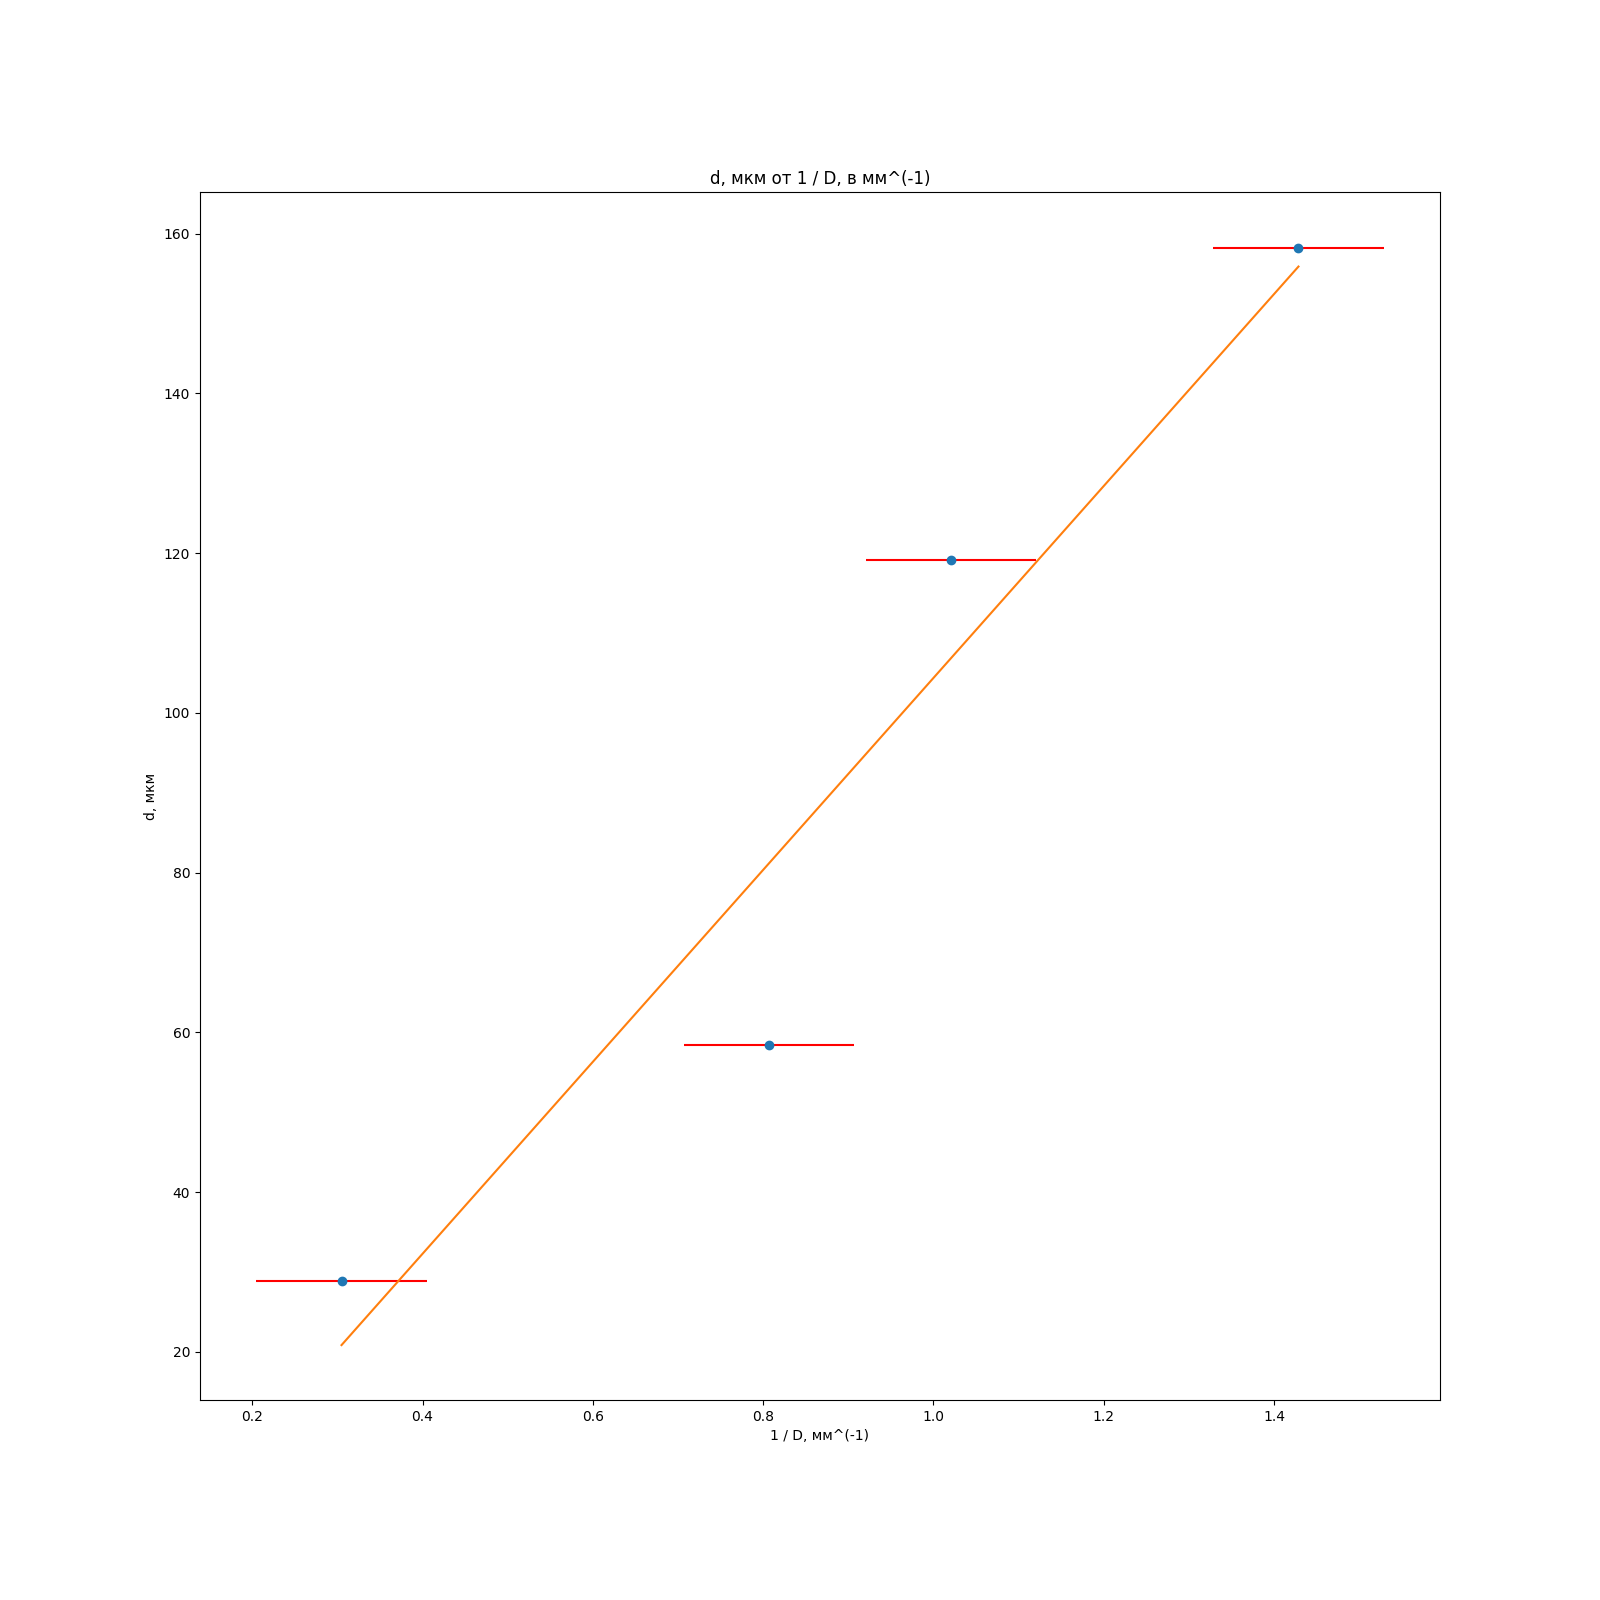
\includegraphics[scale = 0.4]{graph1.png}
        \caption{График зависимости $d = f \left( 1 / D \right)$}
        \label{graph1}
    \end{figure}
\end{enumerate}
\end{document}